\pagestyle{empty}
\cleardoublepage
\pagestyle{fancy}

\chapter{Mancal magnético}

%\begin{small}
%\begin{itemize}
%	\item especificações
%		\begin{itemize}
%			\item massa 
%			\item dimensões
%			\item consumo 
%			\item potência máxima
%		\end{itemize}
%	\item restrições
%	\item introdução da topologia do mancal
%	\item estator externo
%		\begin{itemize}
%			\item ímãs 
%			\item perfil em C
%			\item ferro
%			\item 
%		\end{itemize}
%	\item estator interno
%		\begin{itemize}
%			\item bobinas
%		\end{itemize}
%	\item batente
%	\item base
%	\item fixação ?
%	\item modelo em elementos finitos
%\end{itemize}
%\end{small}

O mancal magnético proposto deve satisfazer as especificações da Sec.  \ref{sec:especificações}, onde se deseja atingir os requisitos de uma roda de reação para um satélite de classe II, baseado nos dados da plataforma multimissão (PMM) do INPE \citep{Veloso2009}, possibilitando que o satélite possa rejeitar pertubações orbitais e executar manobras de posicionamento. 


\section{Especificações} \label{sec:especificações}

O acionamento da roda de reação deve ser possível em ambos os sentidos de rotação e com a mesma eficiência. Requer também que o eixo de rotação tenha inclinação menor do que 0,1 grau com relação à superfície de fixação da roda. A precisão de alinhamento é necessária para a adequada atuação da roda de reação no eixo sob controle.

A roda de reação deve ter dimensões limitadas em 250mm de diâmetro por 100mm de altura com massa total que não deve exceder 4kg. Na concepção das partes construtivas da roda de reação foi considerada a necessidade de operação contínua por longos períodos de tempo (em torno de quatro anos).

A Tab. \ref{tab:PMM:especificações} é um resumo das especificações da roda de reação, nela estão as características mecânicas e elétricas de uma roda de reação especificada pelo Instituto Nacional de Pesquisas Espaciais (INPE).

\begin{table}[!ht]
    \centering
    \begin{tabular}{l c c l }
		Parâmetro & & Valor &   \\
       	\hline \hline
 		Torque   					& nominal	  & 0,1 & [Nm]  \\
 		Momento angular  			& nominal	  & 10 &      [Nms] \\
 		Rotação 					& máxima		  & $\pm4000$ & [rpm] \\
 		Oscilação do torque 		& máximo		  & 10  & [\%] \\
 		Torque de fricção do mancal & máximo		  & 0,01 & [Nm] \\
 		\multirow{2}{*}{Desbalanceamento residual} & estático & 0,2 & [g.cm]\\
 		& dinâmico & 20  & [g.cm$^{2}$]  \\
 		\multirow{3}{*}{Consumo de potência} 
 		& mínima & 3 & [W] 	 \\
 		& nominal & 30 & [W] \\
 		& máxima & 100 & [W] 	\\	
 		Tensão de alimentação  & nominal & 20 à 40 & [V]  \\
    \end{tabular}
    \caption{Especificações de requisito da roda de reação}
    \label{tab:PMM:especificações}
\end{table}

A seguir um explicativo de cada especificação :

\paragraph{Torque:}
A magnitude do torque disponibilizado pela roda de reação determina sua capacidade de atuação em vista de perturbações, e consequentemente o desempenho do sistema controle de atitude. 

\paragraph{Momento Angular:}
A faixa de operação em momento angular determina a capacidade de manobra e o período de operação autônoma das rodas.

\paragraph{Velocidade de Rotação:}
A velocidade máxima de rotação especificada atende a um compromisso de de minimização da massa e das dimensões para o momento máximo desejado, bem como à limitação do jitter de atitude devido ao desbalanceamento do componente de inércia.

\paragraph{Oscilação de Torque:}
A oscilação de torque é indesejável por representar uma limitação para o desempenho do controle de atitude.

\paragraph{Torque de fricção:}
A limitação de torque de fricção visa a minimização de perdas, com impacto na eficiência da roda de reação.


\paragraph{Desbalanceamento residual:} Implica em uma oscilação no eixo de rotação e por consequência gera distúrbios no satélite.

\paragraph{Tensão de Alimentação:} Níveis de alimentação comummente encontrados em satélites.


\section{Visão Geral}

% [Scharfe2001]
% Magnetic bearings can be realised by using attractive or repulsive forces. A better mass vs. stiffness ratio can be achieved by using the attractive force mode. Preference was given to the 2 DOF option where the wheel is actively controlled along two orthogonal radial directions where axial movements and all other degrees of rotor freedom are passively controlled by means of permanent magnets, except for the rotor spin. The two radial axes are independently controlled by their control loops. This design principle generally results in a flatter geometry, using less volume and being suitable for panel mounting. Moreover, the two DOF actively controlled bearing allows a high momentum-to-mass ratio of the wheel as parts of the bearing contribute to the momentum storage capacity. For position detection, magnetic field displacement type inductive sensors are mounted with 90 degrees angular spacing around the flywheel, facing the rim surface.

O mancal magnético proposto neste trabalho é, em parte, uma junção das topologias propostas por \citet{Bernus1998} e \citet{Scharfe2001}. O mancal possui quatro graus de liberdade passivamente estáveis: sendo eles seus deslocamentos angulares (\textit{tilt, roll, pitch}) e seu deslocamento na direção axial, os outros dois graus de liberdade (os deslocamentos radiais) são estabilizados ativamente. O torque imposto para a rotação do rotor não é abordado neste trabalho mas será desenvolvido por um motor elétrico de corrente contínua sem escovas, instalado no interior do mancal.


O circuito magnético do mancal é composto por dois estatores: um interno ao rotor, outro externo. O estator externo é responsável pela estabilização dos graus de liberdade passivos, já o interno por possibilitar o controle das posições radiais. Optou-se por instalar os ímãs no estator externo visando um maior fluxo magnético nos modos passivamente estáveis do mancal, além de visar o melhor balanceamento do rotor (se comparada com a instalação dos ímãs no rotor). A Fig. \ref{fig:mancal:topo} ilustra o mancal proposto. O rotor é a parte móvel do mancal e onde é fixada a parte móvel do motor. Adotou-se uma geometria plana visando uma melhor rigidez nos modos instáveis do mancal, possibilitando também a montagem em modo painel. Optou-se por um mancal externo ao motor para conseguir uma rigidez dentro dos limites de massa e dimensões e que atingisse as especificações  da roda de reação. 


\begin{figure}[ht!]
\centering
%\includegraphics[width=0.6\linewidth]{./Figs/mancais/mancal:topo}
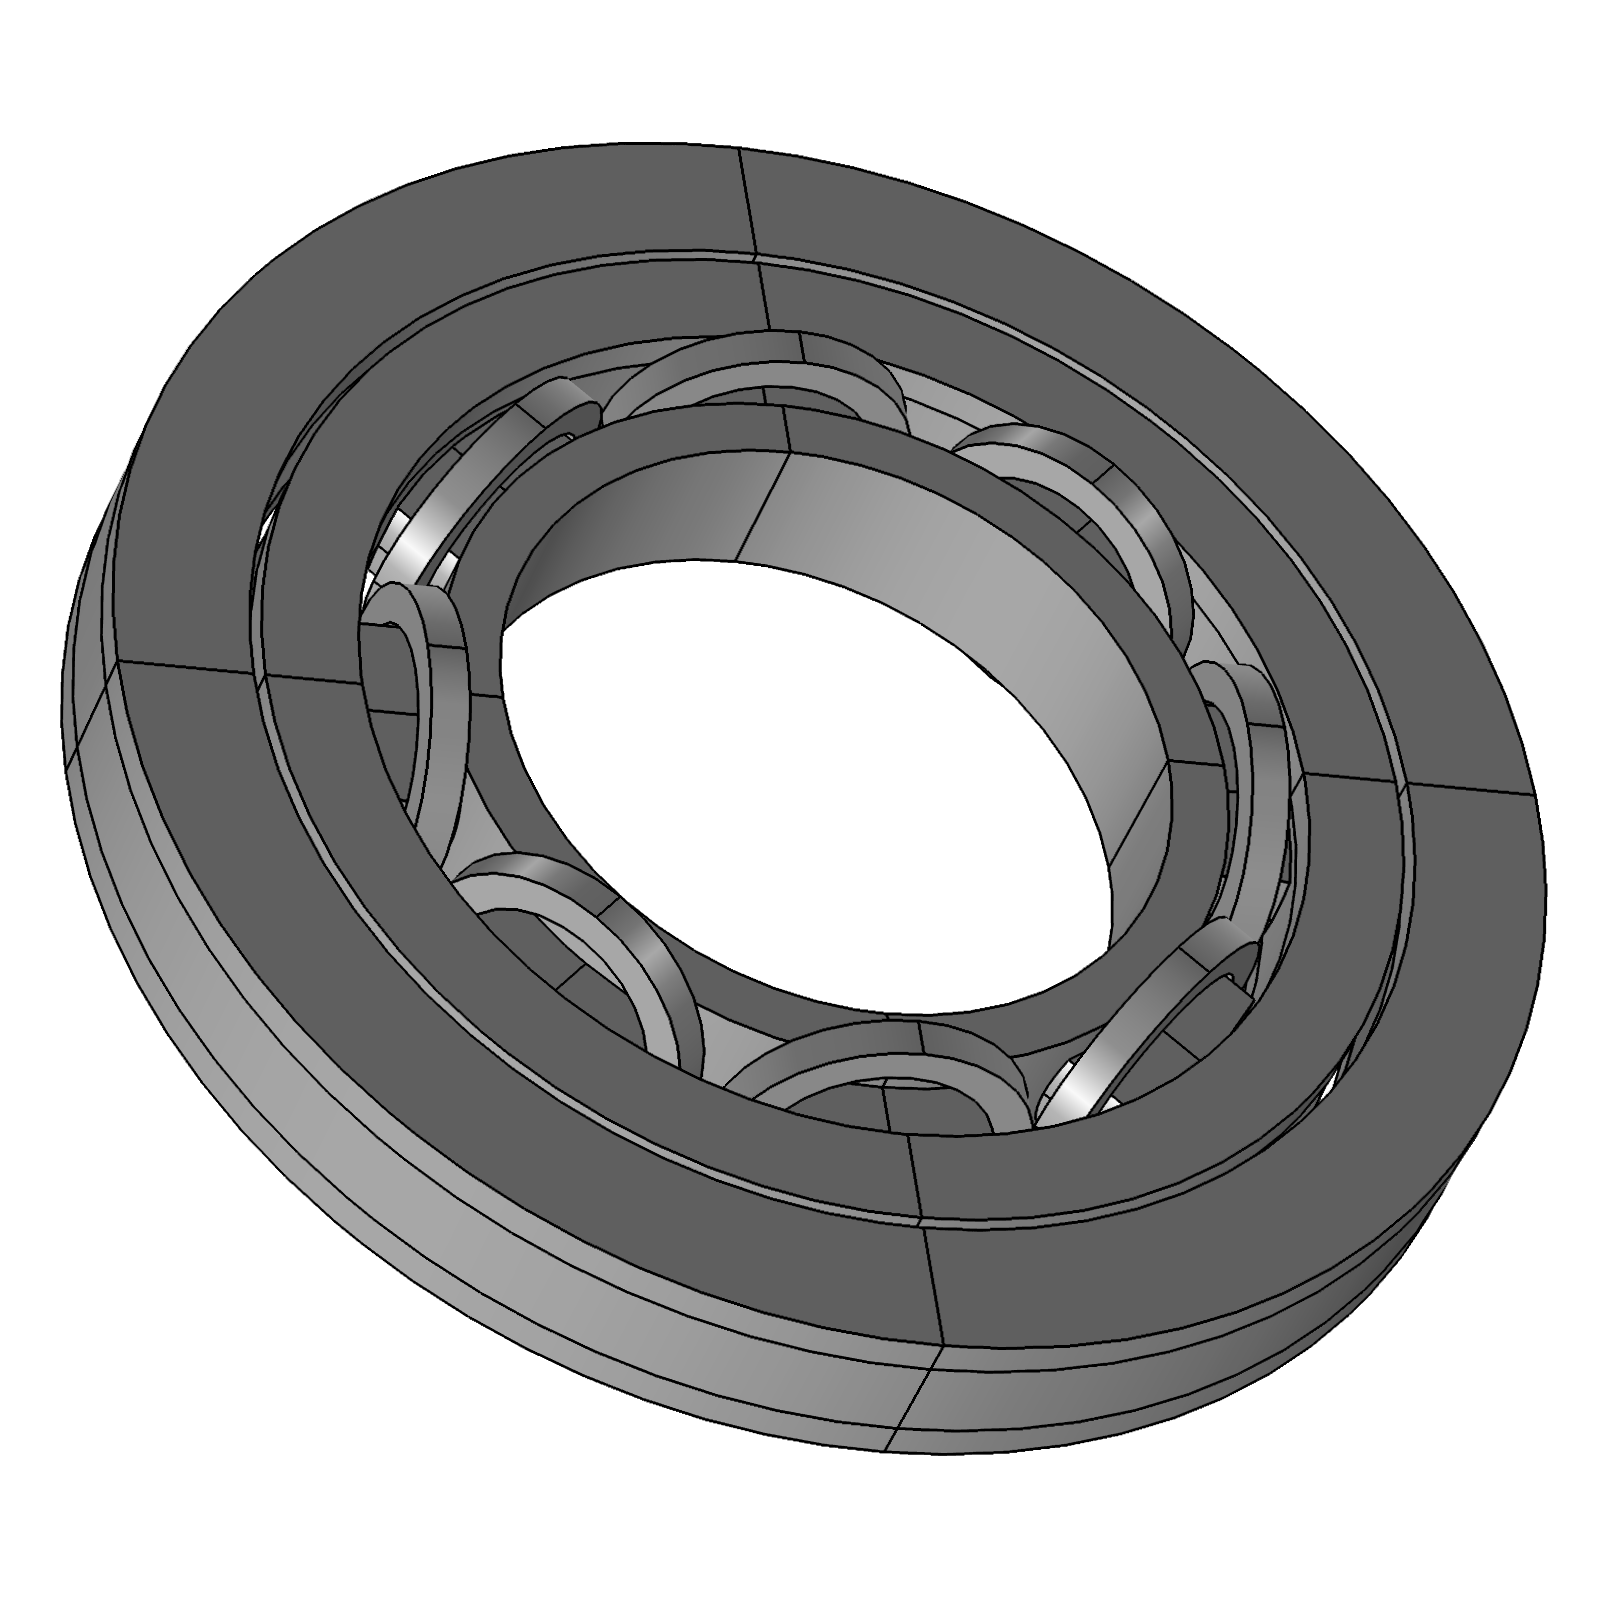
\includegraphics[width=0.6\linewidth]{./mancais/modelo-elementos-finitos}
\caption[Corte ilustrativo do mancal magnético]{Perspectiva das partes magnéticas do mancal}
\label{fig:mancal:topo}
\end{figure}

A Fig. \ref{fig:mancal:corte:radial} e a Fig. \ref{fig:mancal:corte} ilustram consecutivamente os cortes axial e radial do mancal proposto. Verifica-se que os ímãs permanentes estão localizados no estator externo, criando um fluxo magnético que circula pelo rotor e estabiliza o eixo axial.


\begin{figure}[ht!]
	\centering
	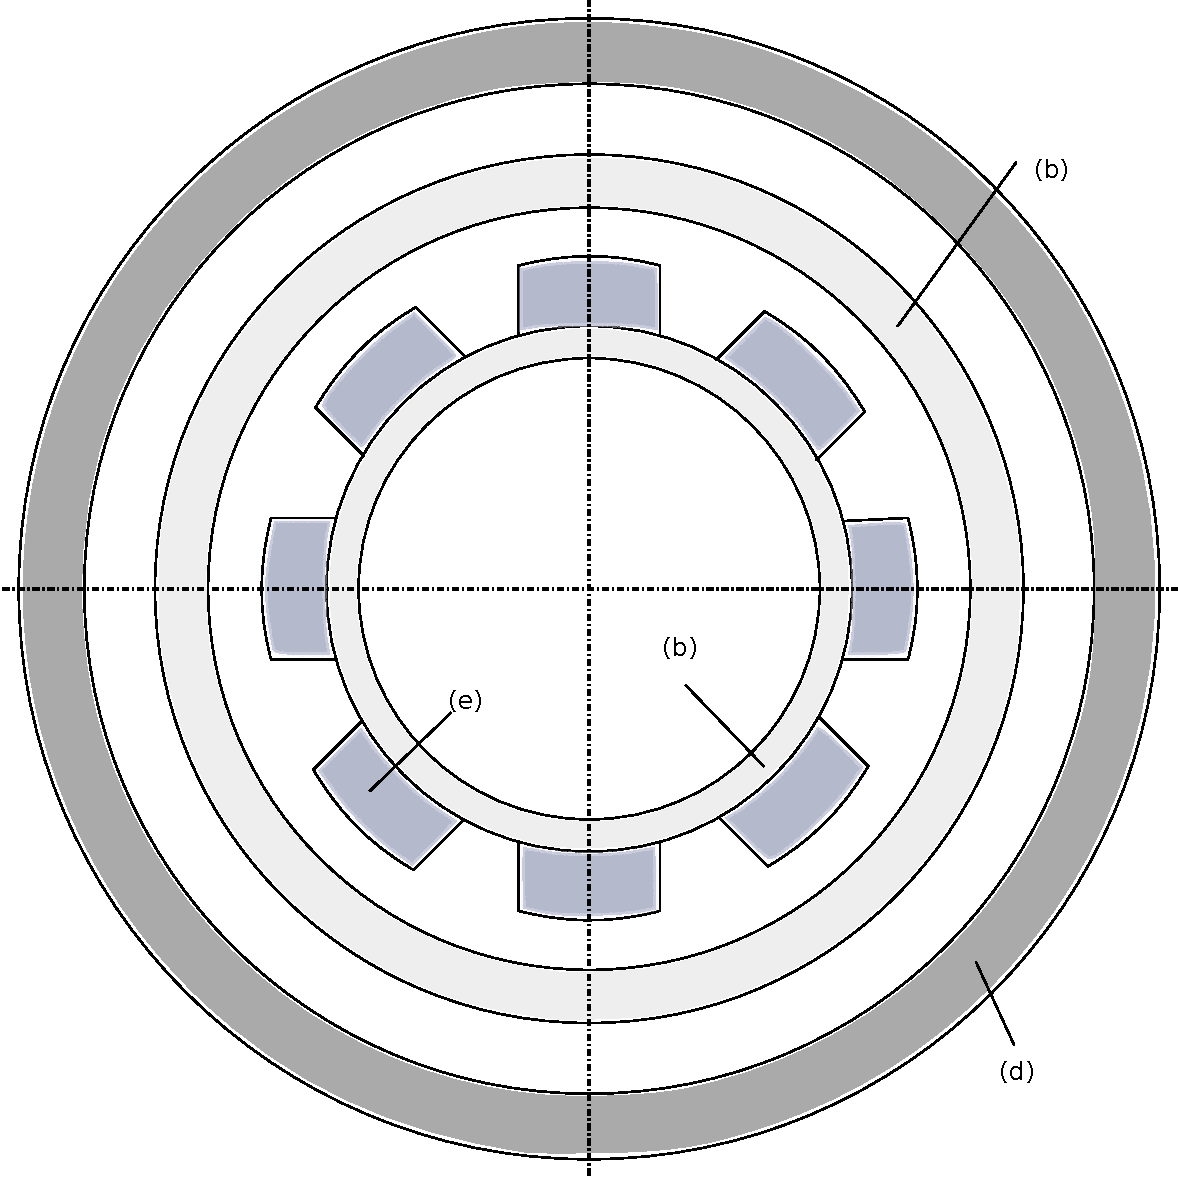
\includegraphics[width=0.7\linewidth]{./Figs/mancais/mancal_corte_radial}
	\caption[Corte radial ilustrativo do mancal magnético]{Corte radial ilustrativo do mancal magnético. Onde:  b) rotor, c) estator interno, d) ímã permanente, e) bobinas}
	\label{fig:mancal:corte:radial}
\end{figure}

Mancais magnéticos podem ser projetados para usar forças magnéticas atrativas ou repulsivas. Uma melhor relação massa/ rigidez pode ser alcançada pela utilização de forças magnéticas atrativas, e este é o papel das bobinas localizadas no estator interno. Oito núcleos são utilizados para exercer força de atração suficiente no rotor para mover da posição de equilíbrio (rotor batido) e estabilizar no ponto de operação. 

\begin{figure}[ht!]
	\centering
	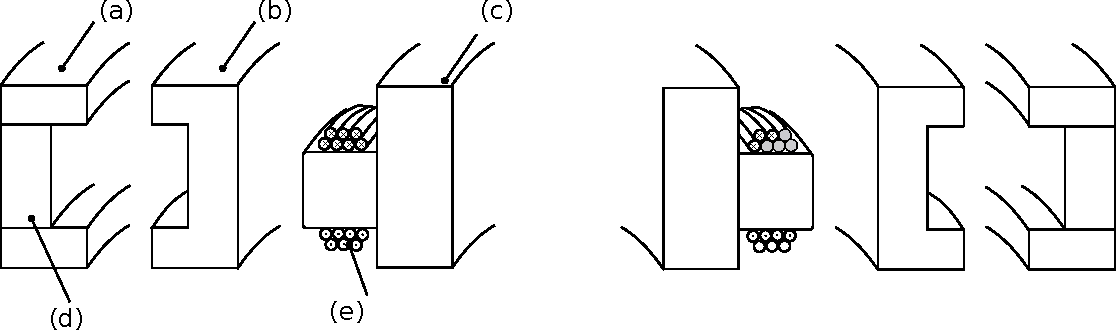
\includegraphics[width=1\linewidth]{./Figs/mancais/mancal_corte}
	\caption[Corte ilustrativo do mancal magnético]{Corte ilustrativo do mancal magnético. Onde: a) estator externo, b) rotor, c) estator interno, d) ímã permanente, e) bobinas}
	\label{fig:mancal:corte}
\end{figure}

Um batente foi projetado para evitar que as partes magnéticas (metálicas) se choquem em caso de falha na malha de controle ou em situações em que o sistema encontra-se desligado. O batente limita a excursão máxima do rotor em seus graus de liberdade: axial, radial e \textit{tilt}. O batente não interfere no circuito magnético do sistema e está localizado no estator externo. Toda parte fixa do sistema está solidária em uma base também não magnética.

Uma eletrônica de acionamento, sensoriamento e processamento foi alocada na parte inferior da base, tornando o sistema compacto. A eletrônica possui \textit{drivers} para controle das correntes nas bobinas e também um sistema de sensoriamento para medir a posição do rotor. Um sistema microprocessado foi proposto para realizar o controle e gestão do sistema.

% O mancal é composto dos seguintes subsistemas:
%
%\begin{itemize}
%	\item estator Interno
%	\item estator Externo
%	\item rotor
%	\item batente
%	\item base
%	\item eletrônica
%\end{itemize}

\section{Estator externo}\label{cap:mancal:estator:externo}

O estator externo, responsável pela estabilização dos graus de liberdade passivamente estáveis, é formado por três partes : ferro topo, ímãs, ferro base. A combinação dessas partes faz com que o estator tenha uma secção em formato de C. Os ferros (topo e base) servem para guiar o campo magnético através do gap e pelo rotor. 

O circuíto magnético de uma secção do estator externo é ilustrado na Fig. \ref{Fig:mancal:circuito:passivo}. Verificamos que o fluxo magnético gerado pelo ímã permanente busca o caminho com menor relutância para fechar o circuito magnético. Esse caminho ocorre pelos ferros do estator externo, passando pelo entreferro e  pelo rotor.

\begin{figure}[!ht]
	\centering
	\def\svgwidth{1\columnwidth}
	\includesvg{mancal_passivo_circuito}
	\caption{Circuíto magnético do estator externo}
	\label{Fig:mancal:circuito:passivo}
\end{figure}

Podemos identificar neste circuito seis principais relutâncias, sendo elas :

\begin{itemize}
	\item $R_{ímã}$ : Relutância do ímã permanente
	\item $R_{disp}$ : Relutância de dispersão 
	\item $R_{ft}$ : Relutância devido ao ferro topo
	\item $R_{gt}$ : Relutância do entreferro superior
	\item $R_{fb}$ : Relutância devido ao ferro base
	\item $R_{gb}$ : Relutância do entreferro inferior	
\end{itemize}

Além das relutâncias, tem-se como fonte geradora de campo magnético o ímã localizado entre os ferros: $F_{ima}$. Devido ao fluxo magnético permanente o rotor sofre atração em ambos os lados, no ponto de equilíbrio, ou seja, com um entreferro simétrico em ambos os lados, a força resultante tenderia a ser nula e o rotor permaneceria em equilíbrio no ponto de operação. 

Esse modo de operação é chamado diferencial e possibilita que a força resultante no rotor devido aos ímãs permanentes torne-se linear. Para tanto, projetou-se o estator externo do mancal para trabalhar sempre com o ferro saturado. Na saturação o valor do campo magnético torna-se praticamente constante para pequenas variações no comprimento do entreferro.

Com isso, o fator da força que é proporcional ao quadrado do campo magnético torna-se praticamente constante, obtendo um força de atração radial no rotor linear com o deslocamento.

Além da linearização obtêm-se um aumento na rigidez axial sem um grande aumento na rigidez radial, o que exigiria uma maior energia da parte ativa para estabilizar o rotor em seu ponto de operação. 

No caso de um deslocamento axial ocorre um aumento no comprimento do entreferro e, por consequência, em sua relutância ($R_{g}$), essa condição foge da zona de menor relutância gerando uma força restaurativa no rotor para restabelecer um circuito com menor relutância magnética.

A Fig. \ref{fig:modelo:circuito:passivo:forcas} ilustra as forças atuantes no rotor em dois cenários diferentes, na primeira (a) com o rotor no ponto de equilíbrio (com o mesmo entreferro ao longo de toda circunferência) e em (b) com o rotor deslocado axialmente. Verificou-se nesse caso que a resultante da força não é nula mas sim possui uma componente em y. Essa componente é a responsável pela estabilização dos graus de liberdade passivos.

\begin{figure}[th!]
\centering
\subfloat[rotor no ponto de equílibro]{
	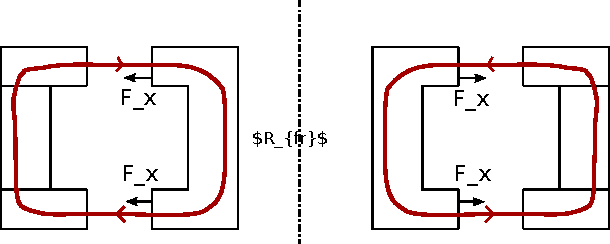
\includegraphics[width=0.8\linewidth]{./Figs/modelo_circuito_passivo_forcas_a}
	} \\
\subfloat[rotor transladado axialmente]{
	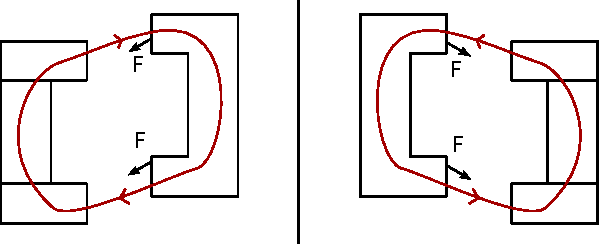
\includegraphics[width=0.8\linewidth]{./Figs/modelo_circuito_passivo_forcas_b}
	}
\caption{Fluxo magnético no estator externo e rotor}
\label{fig:modelo:circuito:passivo:forcas}
\end{figure}

O circuito passivo deve possuir rigidez axial suficiente para manter o rotor alinhado em ambientes com gravidade (para validação em solo) e rigidez radial menor para um baixo gasto energético do circuito ativo na estabilização do rotor.

A estabilidade de inclinação do rotor é garantida pela topologia plana, que prioriza o deslocamento axial ao radial para movimentos angulares.
Com isso, uma pequena inclinação causa um grande deslocamento no eixo z e um pequeno deslocamento nos eixos x e y, gerando um torque restaurativo. 

Caso o mancal não fosse projetado com esse ideal, uma inclinação causaria uma aproximação cruzada dos ferros (rotor e estator externo) tornando o mancal instável ao tilt. 

\section{Rotor}

O rotor foi projetado com perfil em C e sofre tanto a força de atração do estator externo quanto a do interno, porém com campos em diferentes orientações. O rotor é projetado para que seu ferro trabalhe na zona de não saturação; a saturação nesse caso é indesejada pois limitaria o fluxo total através dos circuitos magnéticos e também resultaria, quando em rotação, em uma região de aquecimento e frenagem.

O rotor do mancal magnético deve ser projetado para suportar a fixação do rotor do motor sem escovas assim como a inércia da roda de reação. 

\section{Estator interno}

O estator interno é formado por oito polos distribuídos homogeneamente a cada 45 graus e interligados por um anel de circulação interno. Os polos funcionam como atuadores (eletroímãs) para a estabilização do rotor no eixo radial (x, z);  cada polo é formado por um núcleo. Uma vista em corte de meio mancal é ilustrada na Fig. \ref{fig:modelo:mancal:estator:interno}. 

\begin{figure}[ht!]
	\centering
	\includegraphics[width=1\linewidth]{./Figs/modelo_mancal_estator_interno}
	\caption{Corte em perspectiva do estator interno}
	\label{fig:modelo:mancal:estator:interno}
\end{figure}

O estator interno foi concebido para atuar sempre com três polos ativos por eixo de atuação; essa abordagem faz com que o fluxo do campo magnético que percorre o rotor seja maximizado no eixo onde se deseja realizar a atração. A Fig. \ref{fig:modelo:mancal:estator:interno:fluxo} mostra o caminho do fluxo que flui pelo rotor quando o estator interno opera com três de seus polos ativos: (A),(B),(C) . Os polos (A) e (C) nesse exemplo trabalham com polaridade inversa ao (B) para forçar que o fluxo feche na maior parte por (B) e não por outros polos, maximizando assim a força de atração $F_B$. 

A corrente aplicada nos polos (A) e (C) é por definição do projeto a metade da corrente no polo principal (B). Isso é feito para evitar que o polo (B) opere com um valor elevado do módulo do campo magnético, já que o campo que o atravessa é composto pela totalidade do induzido em sua bobina mais a parte referente aos campos de (A) e (C).

\begin{figure}[ht!]
	\centering
	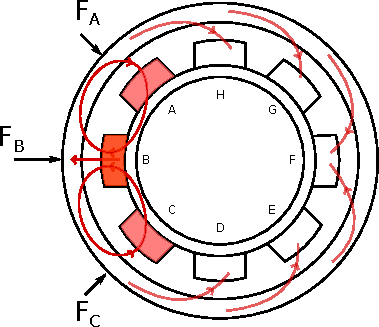
\includegraphics[width=0.7\linewidth]{./Figs/modelo_mancal_estator_interno_fluxo}
	\caption{Fluxo magnético}
	\label{fig:modelo:mancal:estator:interno:fluxo}
\end{figure}

As forças geradas $F_A$ e $F_C$ possuem componentes em x e y; as componentes y são de mesma intensidade e se cancelam, restando uma componente aditiva em x. As forças resultantes são portanto:

\begin{align}
 	F_x &= F_B + F_{Ax} + F_{Cx} \\
 	F_y &= 0 = F_{Cy} - F_{Ay} 
\end{align}


Nesse modo de operação pode-se gerar forças exclusiva em apenas um dos eixos (x,y). É possível também atuar simultaneamente nos dois eixos, para isso basta induzir da mesma maneira um novo campo em (H) e (G). Desse modo, o campo total no núcleo da bobina (A) será equivalente ao dos polos primários. A Fig. \ref{fig:modelo:mancal:estator:interno:fluxo2} ilustra o campo magnético e as forças resultantes geradas no caso da atuação simultânea.

 \begin{figure}[ht!]
 	\centering
 	\includegraphics[width=0.7\linewidth]{./Figs/modelo_mancal_estator_interno_fluxo2}
 	\caption{Fluxo magnético}
 	\label{fig:modelo:mancal:estator:interno:fluxo2}
 \end{figure}

O circuito magnético entre o estator interno e o rotor pode ser visto na Fig. \ref{fig:modelo:circuito:ativo:explicativo}. Verifica-se que o circuito é formado de quatro principais elementos: a bobina, fonte geradora de campo magnético (c), a relutância do entreferro, que depende da distância entre os polos e o rotor (b), as relutâncias do ferro do rotor (a) e do ferro do anel de retorno (d).

\begin{figure}[ht!]
\centering
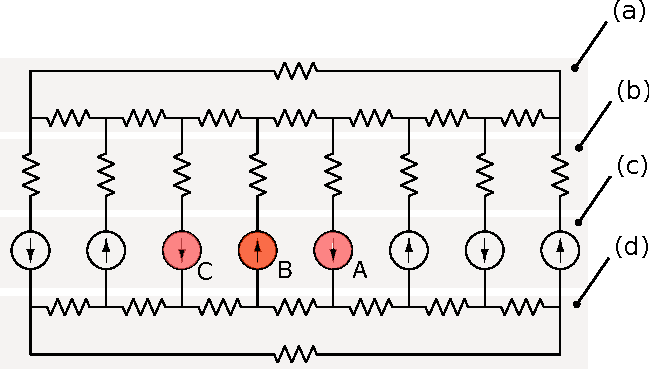
\includegraphics[width=0.7\linewidth]{./Figs/modelo_circuito_ativo_explicativo}
\caption[Circuito eletromagnético estator interno e rotor]{Circuito eletromagnético estator interno e rotor: (a) relutâncias do rotor, (b) relutâncias do entreferro, (c) } 
\label{fig:modelo:circuito:ativo:explicativo}
\end{figure}

Dois tipos de acionamento e embobinamento podem ser realizados para a implementação do atuador. O primeiro considera independência de cada polo, possuindo uma eletrônica exclusiva para o seu acionamento. O segundo, envolve a criação de uma única bobina por atuador, similar aos polos de um motor elétrico onde o mesmo fio é compartilhado entre o polo primário e os polos secundários, resultando em uma bobina de maior resistência e indutância. 

A vantagem da escolha do segundo método seria a simplificação da eletrônica já que seriam necessárias apenas quatro eletrônicas de potência para a atuação, porém implicaria em uma dinâmica mais lenta do atuador visto que as indutâncias seriam associadas em série.

Escolheu-se, neste projeto, trabalhar com eletrônicas de acionamento independente para cada polo, privilegiando assim um atuador com dinâmica mais rápida. Além da dinâmica, possibilita-se dessa maneira que futuros controladores atuem não só nos eixos principais (x,y) (duas entradas) mas também podendo atuar na diagonal (quatro entradas). 

\section{Batente}

 O batente é necessário por duas razões principais: evitar que, caso haja uma falha na estabilização do rotor, as partes metálicas colidam, e também limitar o tamanho máximo do entreferro, limitando por consequência a força de atração máxima que é exercida sobre o rotor.  Essa é necessária para a situação em que o rotor encontra-se mais afastado do ponto de operação, sem o limite do batente o entreferro se tornaria grande o que exigiria uma potência maior das bobinas para estabilizá-lo no ponto de operação.  Além de limitar a máxima translação radial, o batente é responsável por limitar também a translação axial e sua inclinação (\textit{tilt}).
 
 A Fig. \ref{fig:mancal:batente:corte} é uma ilustração do batente proposto para o mancal magnético. Este é composto de duas partes: (a) responsável por limitar o entreferro máximo entre o rotor e o estator externo; (b) flange para limitar a inclinação do rotor. Encontra-se na literatura projetos de mancais magnéticos com rolamentos. Essa escolha seria inadequada para o projeto já que a proposta é a aproximação de um projeto espacializável e a incorporação do rolamento demandaria um projeto específico.
 
Optou-se por instalar o batente no estator externo por duas razões distintas: facilidade na montagem, pois  é o local que possui maior entreferro (portanto espaço) e também para servir de fixação para unir os ímãs e os ferros do estator externo. 

\begin{figure}[th!]
\centering
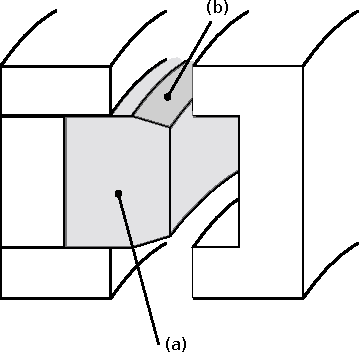
\includegraphics[width=0.4\linewidth]{./Figs/mancais/mancal_batente_corte}
\caption{Ilustração do batente proposto}
\label{fig:mancal:batente:corte}
\end{figure}


O batente deve ser rígido o suficiente para suportar possíveis impactos do rotor. Será visto no Cap. \ref{Cap:Modelagem:Dinamica} que essas forças são da ordem de centenas de Newtons. A utilização de Nylon ou Teflon na construção do batente é aconselhável \citep[Cap. 13]{Schweitzer2009} devido às suas propriedades de lubrificação a seco e absorção a impacto.

\section{Base}

As partes não móveis do mancal são fixas em uma base de propriedade não magnéticas (alumínio), a base serve para alinhar as partes do mancal e ao mesmo tempo possibilita a movimentação do rotor na direção axial e radial (dentro das especificações de oscilação). 

%\section{Eletrônica}
%
%A eletrônica proposta é composta de sistemas de potência para o acionamento das bobinas (polos), eletrônica de sensoriamento para medição das posições do rotor e uma eletrônica de controle (digital) onde é implementado o controle do sistema. 

%Um sistema microconrolado (ou FPGA) é proposto para implementação das leis de controle, o acionamento das bobinas será realizado através da modulação da largura de pulso (PWM).

\section{Dimensões}

Ao longo do desenvolvimento da dissertação, as nomenclaturas a seguir foram utilizadas para descrever as dimensões do mancal proposto. As nomenclaturas são esclarecidas na Fig. \ref{fig:modelo_dimensoes} e na Tabela \ref{tab:modelo:dimensoes:nomenclatura}.

\begin{table}[ht!]
	\centering
	\begin{tabular}{c l}
		Símbolo & Descritivo \\
		$h_{fee}$	& Altura do ferro estator externo \\
		$w_{fee}$	& Largura do ferro estator externo\\
		
		$h_m$		& Altura do ímã \\
		$w_m$		& Largura do ímã \\

		$g_{ne}$	& Entreferro nominal externo \\
		
		$w_{fr}$	& Largura do ferro rotor \\
		
		$g_{ni}$	& Entreferro nominal interno \\
		
		$h_n$		& Altura do polo da bobina \\
		$w_n$		& Largura do polo da bobina \\
		
		$w_{fei}$	& Largura do ferro estator interno \\
		$h_{fei}$	& Altura do ferro estator interno \\

		$r_{eei}$	& Raio do polo estator externo \\				
		$r_{re}$	& Raio do polo do ferro rotor \\		
		$r_{n}$		& Raio do polo da bobina \\		
		$r_{ei}$	& Raio do ferro estator interno \\		
		
	\end{tabular} 
	\caption{Símbolos utilizados na descrição do mancal}
	\label{tab:modelo:dimensoes:nomenclatura}
\end{table}


\begin{figure}[th!]
	\centering
	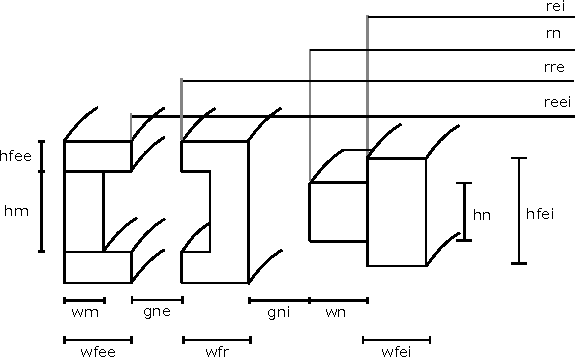
\includegraphics[width=0.8\linewidth]{Figs/modelo_dimensoes}
	\caption{}
	\label{fig:modelo_dimensoes}
\end{figure}

 \section{Modelo em Elementos Finitos}
 
 Foi utilizado como ferramenta de modelagem o Software de elementos finitos e multi-física \textit{Comsol}. Nas simulações, foram utilizados a curva de histerese do Aço 1020 , as simulações foram realizadas com um sólido tridimensional e a análise realizada foi a estacionária.  A Fig. \ref{Fig:Simulacao:Passivo:Mesh} ilustra a malha utilizada na execução das simulações com um número aproximado de 19000 elementos.
 
 \begin{figure}[!ht]
 	\centering
 	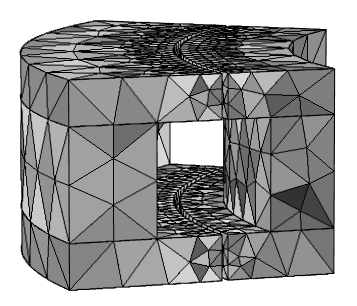
\includegraphics[width=0.5 \columnwidth,angle=0]{Figs/Simulacoes/Passivo/3D_Mesh=1,2.png}
 	\caption{Modelo Comsol do circuito passivo Malha utilizada nos cálculos}
 	\label{Fig:Simulacao:Passivo:Mesh}
 \end{figure}
 
Nas simulações em elementos finitos, o modelo criado utiliza físicas distintas para os diversos elementos do mancal. No caso dos ferros, aplicou-se a lei de Ampère com a relação \textbf{BH} interpolada de uma tabela \citep{MagWeb2015}. Nos componentes compostos por ar, a relação utilizada foi a linear $B=\mu_0 H$. 

Na simulação do ímã, utilizou-se a relação de magnetização  $B = \mu_0 (H + M)$ onde M é a magnetização do meio em A/m. Para as bobinas, o material utilizado foi o cobre e a equação para a densidade de corrente (J) aplicada foi: $ J = \frac{N I}{A}$, onde: $N$ é o número de espiras, $I$ a corrente total aplicada na bobina e $A$ a área da secção da bobina.

Optou-se por trabalhar com o mancal em três dimensões para a obtenção de um modelo de forças e campos magnéticos mais precisos, porém, em contra partida, o tempo para convergência dos resultados implicou em uma simulação relativamente demorada (10 minutos) em um computador com processador Intel i7 e 16G de memória volátil (RAM).

\section{Prototipagem}
 
Para a prototipagem do mancal foi necessário a criação de nove diferentes peças que possibilitassem a montagem do sistema. A proposta de montagem visou minimizar a influência no circuito magnético que alteraria o comportamento das forças no rotor mas, ao mesmo tempo, buscou-se um sistema simétrico e robusto.  A Fig. \ref{fig:montgem:corte} é um corte da estrutura proposta, verificou-se que o estator interno (RW-M-EI) é formado por uma única peça, enquanto o rotor e o estator externo são fragmentados em mais de uma parte.

A Tab. \ref{Tab:nomenclatura:mancal} possui a descrição e nomenclatura das partes propostas para a prototipagem do mancal magnético.

 \begin{table}[ht!]
 	\centering
 	\begin{tabular}{l l}
 		Nomenclatura & Descrição  \\ \hline
 		RW-M-BA 		&	Base do mancal \\
 		RW-M-C   		 &	Casca externa\\
 		RW-M-EEB	  & Estator externo base\\
 		RW-M-EET & 	Estator externo topo\\
 		RW-M-BT & 	Batente\\
 		RW-M-RFB & 	Rotor ferro base\\
 		RW-M-RFT	&  Rotor ferro topo\\
 		RW-M-RN & 	Rotor núcleo\\
 		RW-M-EI	&  Estator interno\\
		RW-M-IM	&  Ímãs 
 	\end{tabular} 
 	\caption{Nomenclatura partes mancal}
 	\label{Tab:nomenclatura:mancal} 
 \end{table} 

 
A não utilização de materiais laminados propicia a aparição de correntes parasitas de Foucault no circuito magnético, quando exposto a correntes variantes no tempo. Essas correntes induzidas  causam uma redução na força eletromagnética e aquecem o material, alterando a relação corrente/força utilizada como parâmetro para o projeto da lei de controle. Minimizar as correntes induzidas tornam o sistema mais eficiente porém a construção de um protótipo laminado é mecanicamente difícil. Outra solução é a utilização de \textit{soft iron} \citep{Boglietti2003}, que possui propriedades que limitam a criação de corrente induzida. Em contrapartida, esses materiais normalmente apresentam menor permeabilidade magnética e menor valor do campo magnético para atingir a saturação \citep{Han2013a}. O material escolhido para os circuitos magnéticos foi o Aço 1020 e para as partes não magnéticas utilizou-se o alumínio.
  
\begin{figure}[th!]
\centering
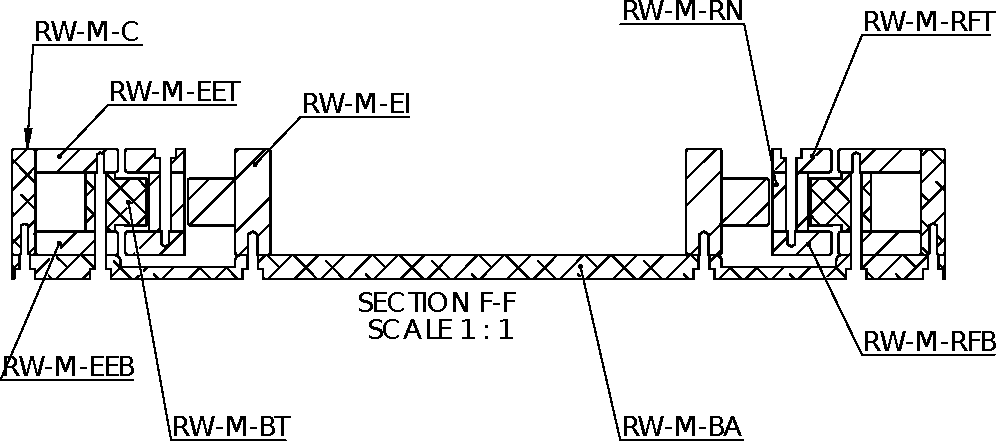
\includegraphics[width=1\linewidth]{./mancais/montgem_corte}
\caption{Partes do mancal}
\label{fig:montgem:corte}
\end{figure} 

A escolha da localização e dos tipos de parafuso (magnético, não magnético) foi uma decisão de projeto, optou-se por uma localização que minimizasse a influência no circuito magnético, no caso do estator interno e utilizou-se parafusos com materiais magnéticos alinhados com os polos. Verificou-se que essa região é a que menos impacta nos campos magnéticos (analisado via elementos finitos).

No caso da fixação do estator externo, utilizou-se parafusos não magnéticos, caso contrário seriam um caminho não desejado para as linhas de campo. As partes do rotor foram montadas com parafusos magnéticos.

A prototipagem foi realizada para a verificação da arquitetura proposta analisando as estabilidades passivas e as demais forças envolvidas. Esse protótipo foi construído a partir de um estudo inicial e não possui as dimensões otimizadas encontradas nos capítulos seguintes, porém suas dimensões são da ordem de grandeza do resultado desta dissertação.

Dificuldades foram enfrentadas com essa versão, dentre elas a do embobinamento dos polos. Devido ao espaço restrito, não se conseguiu via métodos manuais alcançar a quantidade de bobinas prevista no projeto teórico, impossibilitando o teste da força de atração do estator interno.

A falta de precisão na usinagem causou desalinhamento das peças e diferença nos raios, dificultando a montagem. Na concepção inicial do protótipo, uma casca externa foi projetada (RM-M-C) para fixar os ímãs e impedir que eles fossem expelidos radialmente, mas devido às imprecisões mecânicas dos ímãs (causadas pelo banho de níquel) não foi possível a utilização dessa peça. 

A Fig. \ref{fig:partes} e \ref{fig:completo} é uma imagem das partes construídas do mancal magnético, a primeira, com as partes desmontadas e a segunda com o mancal montado.


\begin{figure}[ht!]
\centering
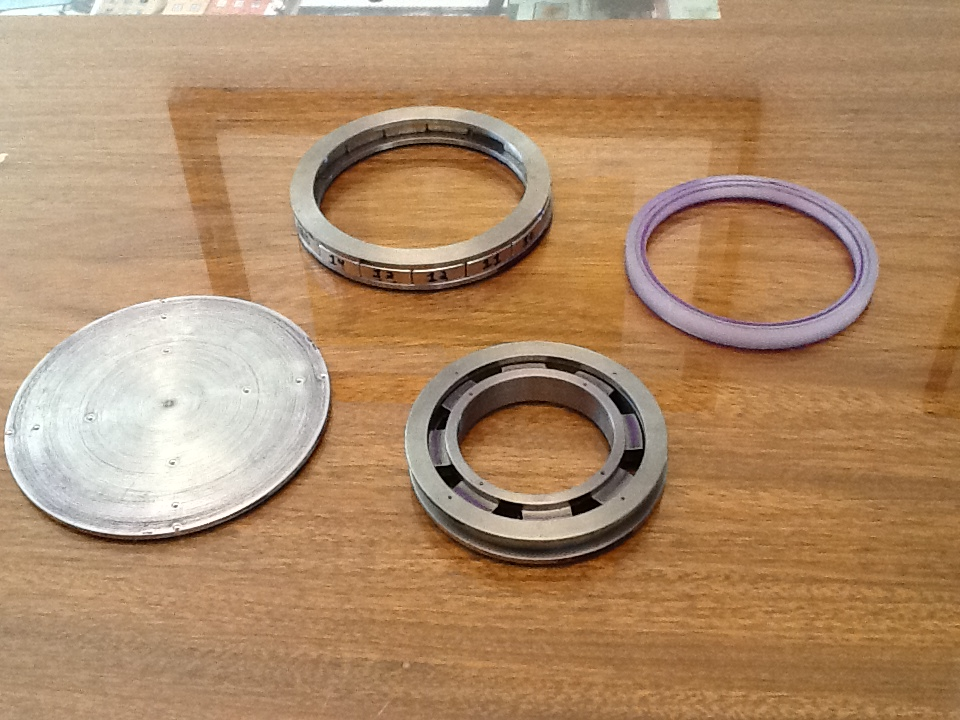
\includegraphics[width=0.8\linewidth]{Figs/img/partes}
\caption{Componentes do protótipo}
\label{fig:partes}
\end{figure}


\begin{figure}[ht!]
\centering
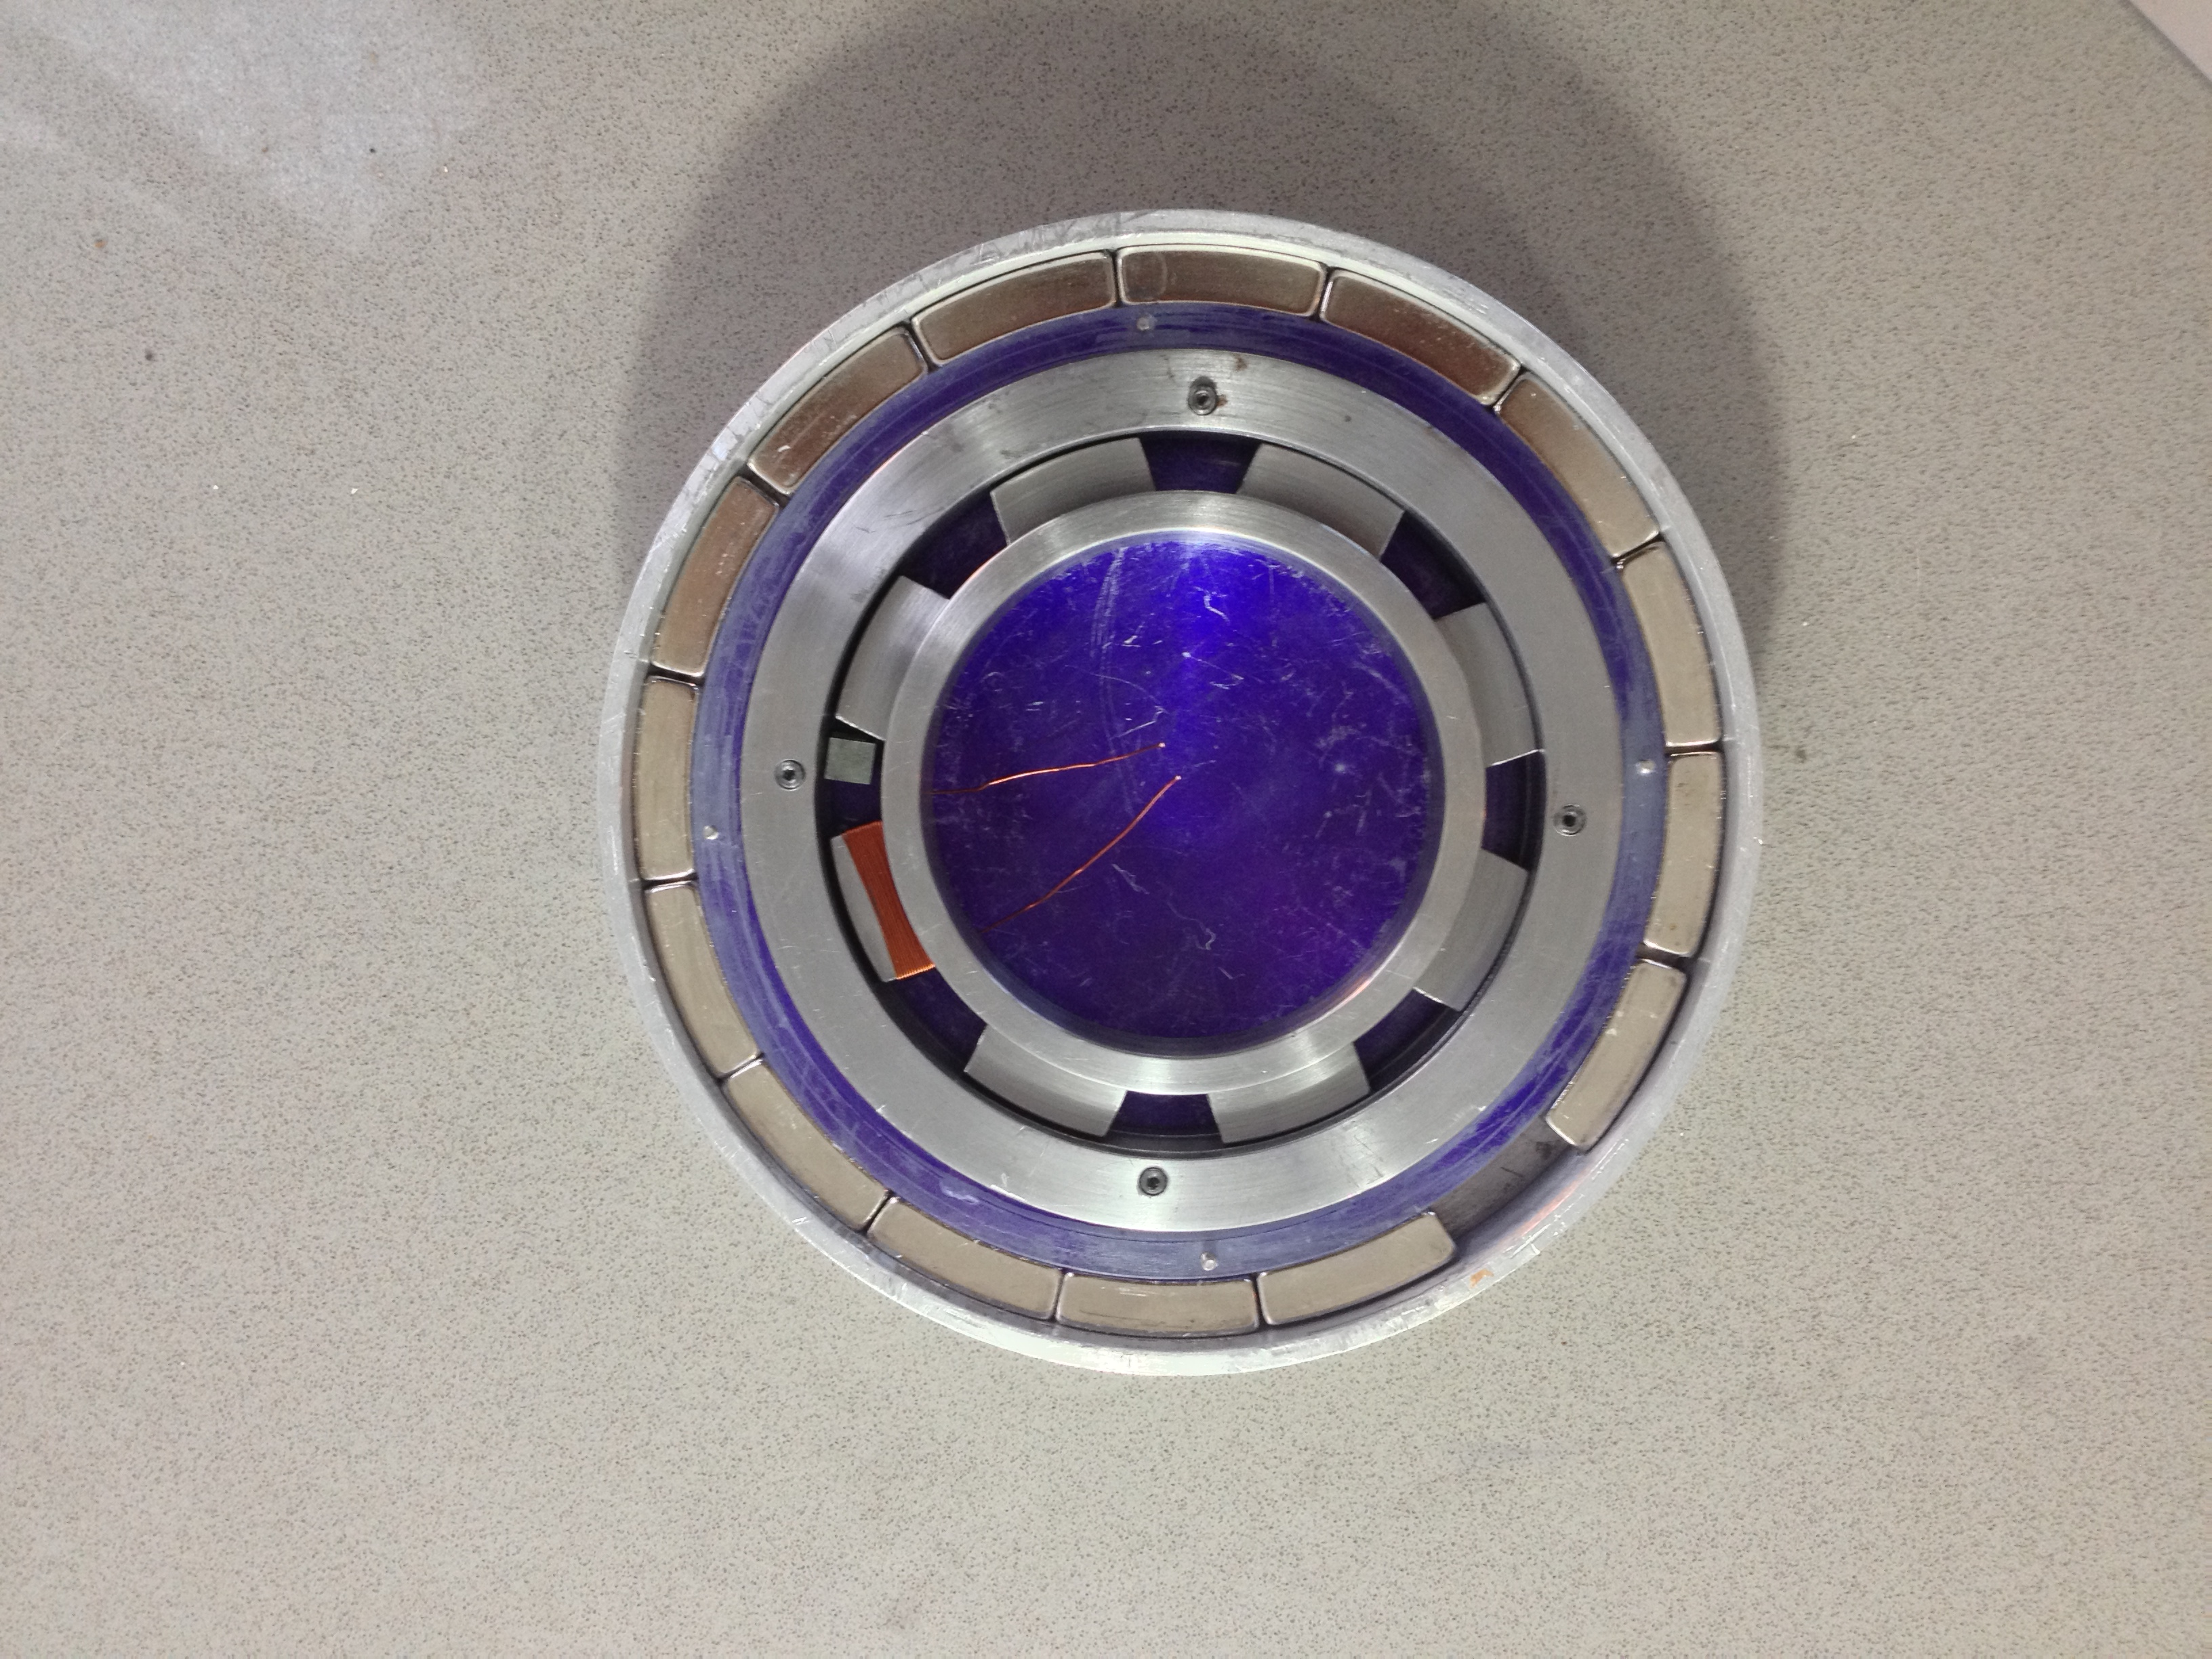
\includegraphics[width=0.8\linewidth]{Figs/img/completo}
\caption{Protótipo montado, vista superior}
\label{fig:completo}
\end{figure}


